\section{Photonic Front-End}
The working principle of the optic time-stretch technique can be described in two steps (see \autoref{fig:eo_ts}).
First, a short laser pulse is propagated in a dispersive medium (optical fiber of length $L_1$). %todo EOSD?
This results in a chirped laser pulse of the duration
\begin{equation}
	T_1 = \Delta \lambda D_1 L_1
\end{equation}
with the optical bandwidth of the laser pulse $\Delta \lambda$  and the dispersion parameter $D_1$ of the fiber.
The next step is the time-to-wavelength-mapping, where a temporal intensity modulation is imprinted on the chirped pulse.
After that, the modulated chirped pulse propagates through another dispersive medium, a fiber of the length $L_2$.
In this way, the temporal modulation of the pulse is further stretched to the duration $T_2$, which is long enough for detection with photodetectors and/or digitizing with \Glspl{adc}. \cite{roussel2014}

The factor, by which the pulse is slowed down, is calculated as
\begin{equation}
	M = 1 + \frac{L_1}{L_2}.
\end{equation}

\begin{figure}[tbh]
	\centering
	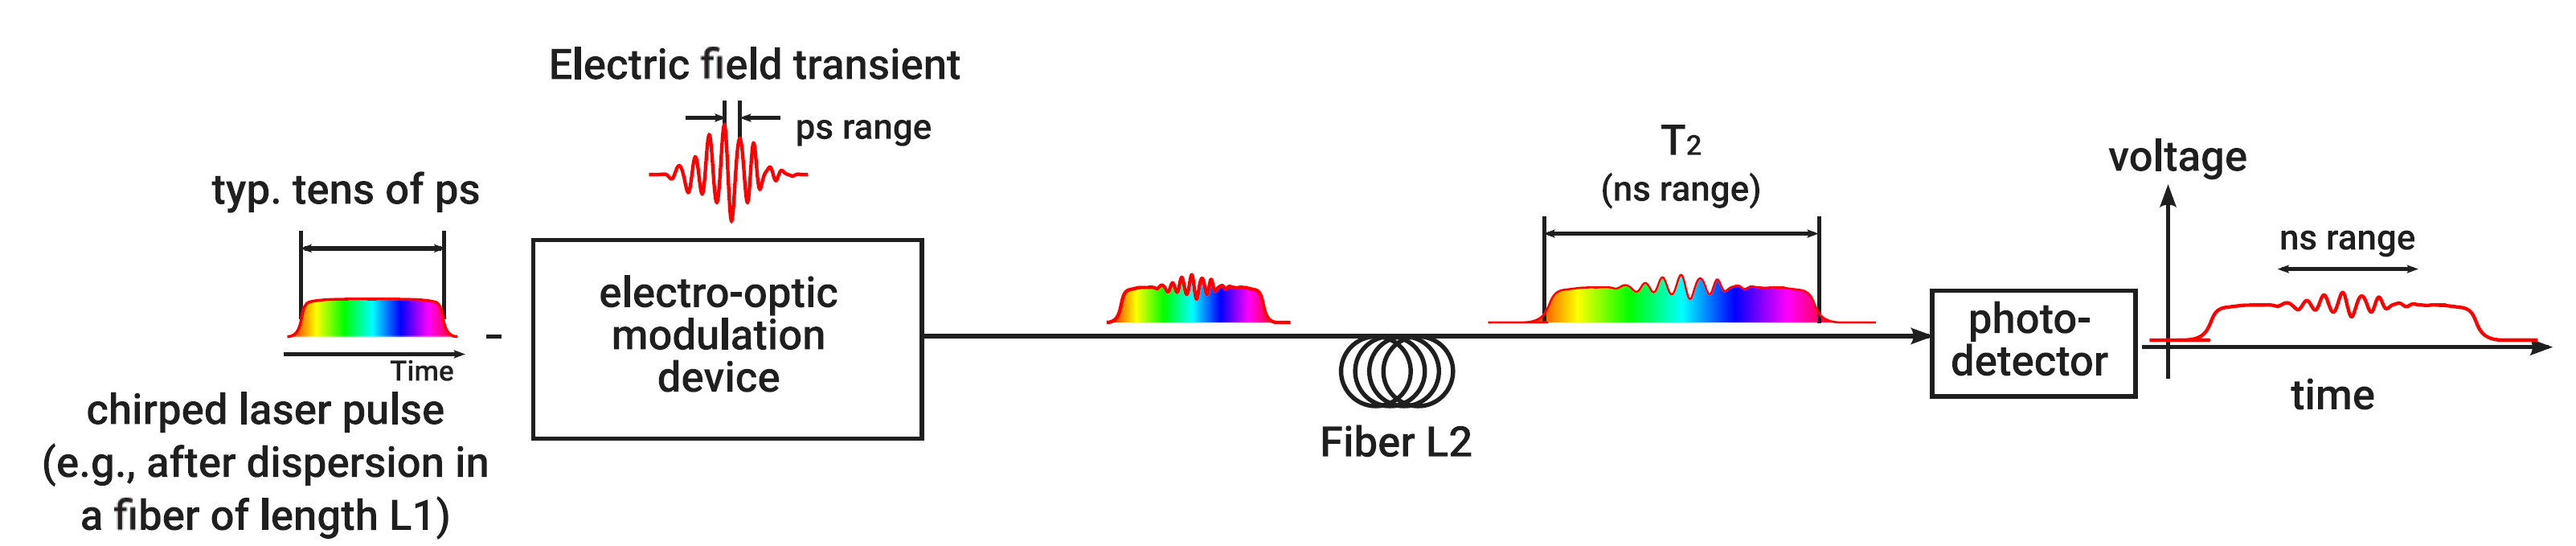
\includegraphics[width = \textwidth]{chap/02-theory/img/time_stretch.png}
	\caption{Electro-Optical Time-Stretch Technique \cite{szwaj}}
	\label{fig:eo_ts}
\end{figure}
%todo at least re-add labels in the figure with tikz, or they are too small


\subsection{Detector/Diode}

The detection and subtraction between the two stretched signals is performed using a amplified balanced photodetector (photoreceiver) from Discovery Semiconductors, with 20 GHz bandwidth and 2800 V/W gain (specified at 1500 nm). The two differential outputs of the detector are sent on a Lecroy LabMaster 10i oscilloscope with 36 GHz bandwidth, 80 GS/s sample rate on each channel and a memory of 256 Mega samples.

\section{Analog-To-Digital Converters}
\Glspl{adc} are used to translate analog quantities into digital signals, which can be processed by information processing, computing, data transmission and control systems. The translation can be seen as encoding a continuous-time analog input (voltage) into a series of discrete, $N$-bit words. This process, which is also called \textit{sampling}, can be expressed as
\begin{equation}
	V_{\text{In}} = V_{\text{FS}} \sum_{k = 0}^{N-1} \frac{b_k}{2^{k+1}} + \epsilon
\end{equation}
with $V_{\text{In}}$ being the input voltage, $V_{\text{FS}}$ the full-scale voltage, $b_k$ the individual output bits and $\epsilon$ the quantization error. \autoref{fig:idealADC} shows the ideal transfer function of a 3-bit \gls{adc}.
\begin{figure}[H]
	\centering
	\includegraphics[width = 0.55\textwidth]{chap/02-theory/img/ideal_adc}
	\caption[Transfer function of ideal, 3-bit ADC]{Transfer function of an ideal, 3-bit \gls{adc} (redrawn from \cite{Lundberg})}
	\label{fig:idealADC}
\end{figure}
%todo what is an ADC, why do we need one in general?

\subsection{Sampling Theory}
An \gls{adc} samples an analog signal with a sample frequency $f_s$.
This frequency has to be chosen in such way, that the original signal can be fully reconstructed.
The \textit{Nyquist criteria} states, that in order to accurately represent a band-limited, continuous signal %todo what is B?
%todo rewrite the condition, maybe like 
\begin{equation}
	y (t) \, \fourier  Y(f) \quad \text{with} \quad Y(f)=0\vert_{f>B/2}
\end{equation}
it has to be sampled with a frequency $f_s$ respecting
\begin{equation}
	f_s > B \quad \text{or} \quad f_s > 2 f_a
\end{equation}
with $f_a$ being the highest frequency contained in the signal. \cite{walt,puente2015}
%todo why not relate f_a to B?

Violation of this rule leads to \textit{aliasing}.
%todo explain aliasing


\begin{figure}[tbh]
	\centering
	\begin{subfigure}{\textwidth}
		\centering
		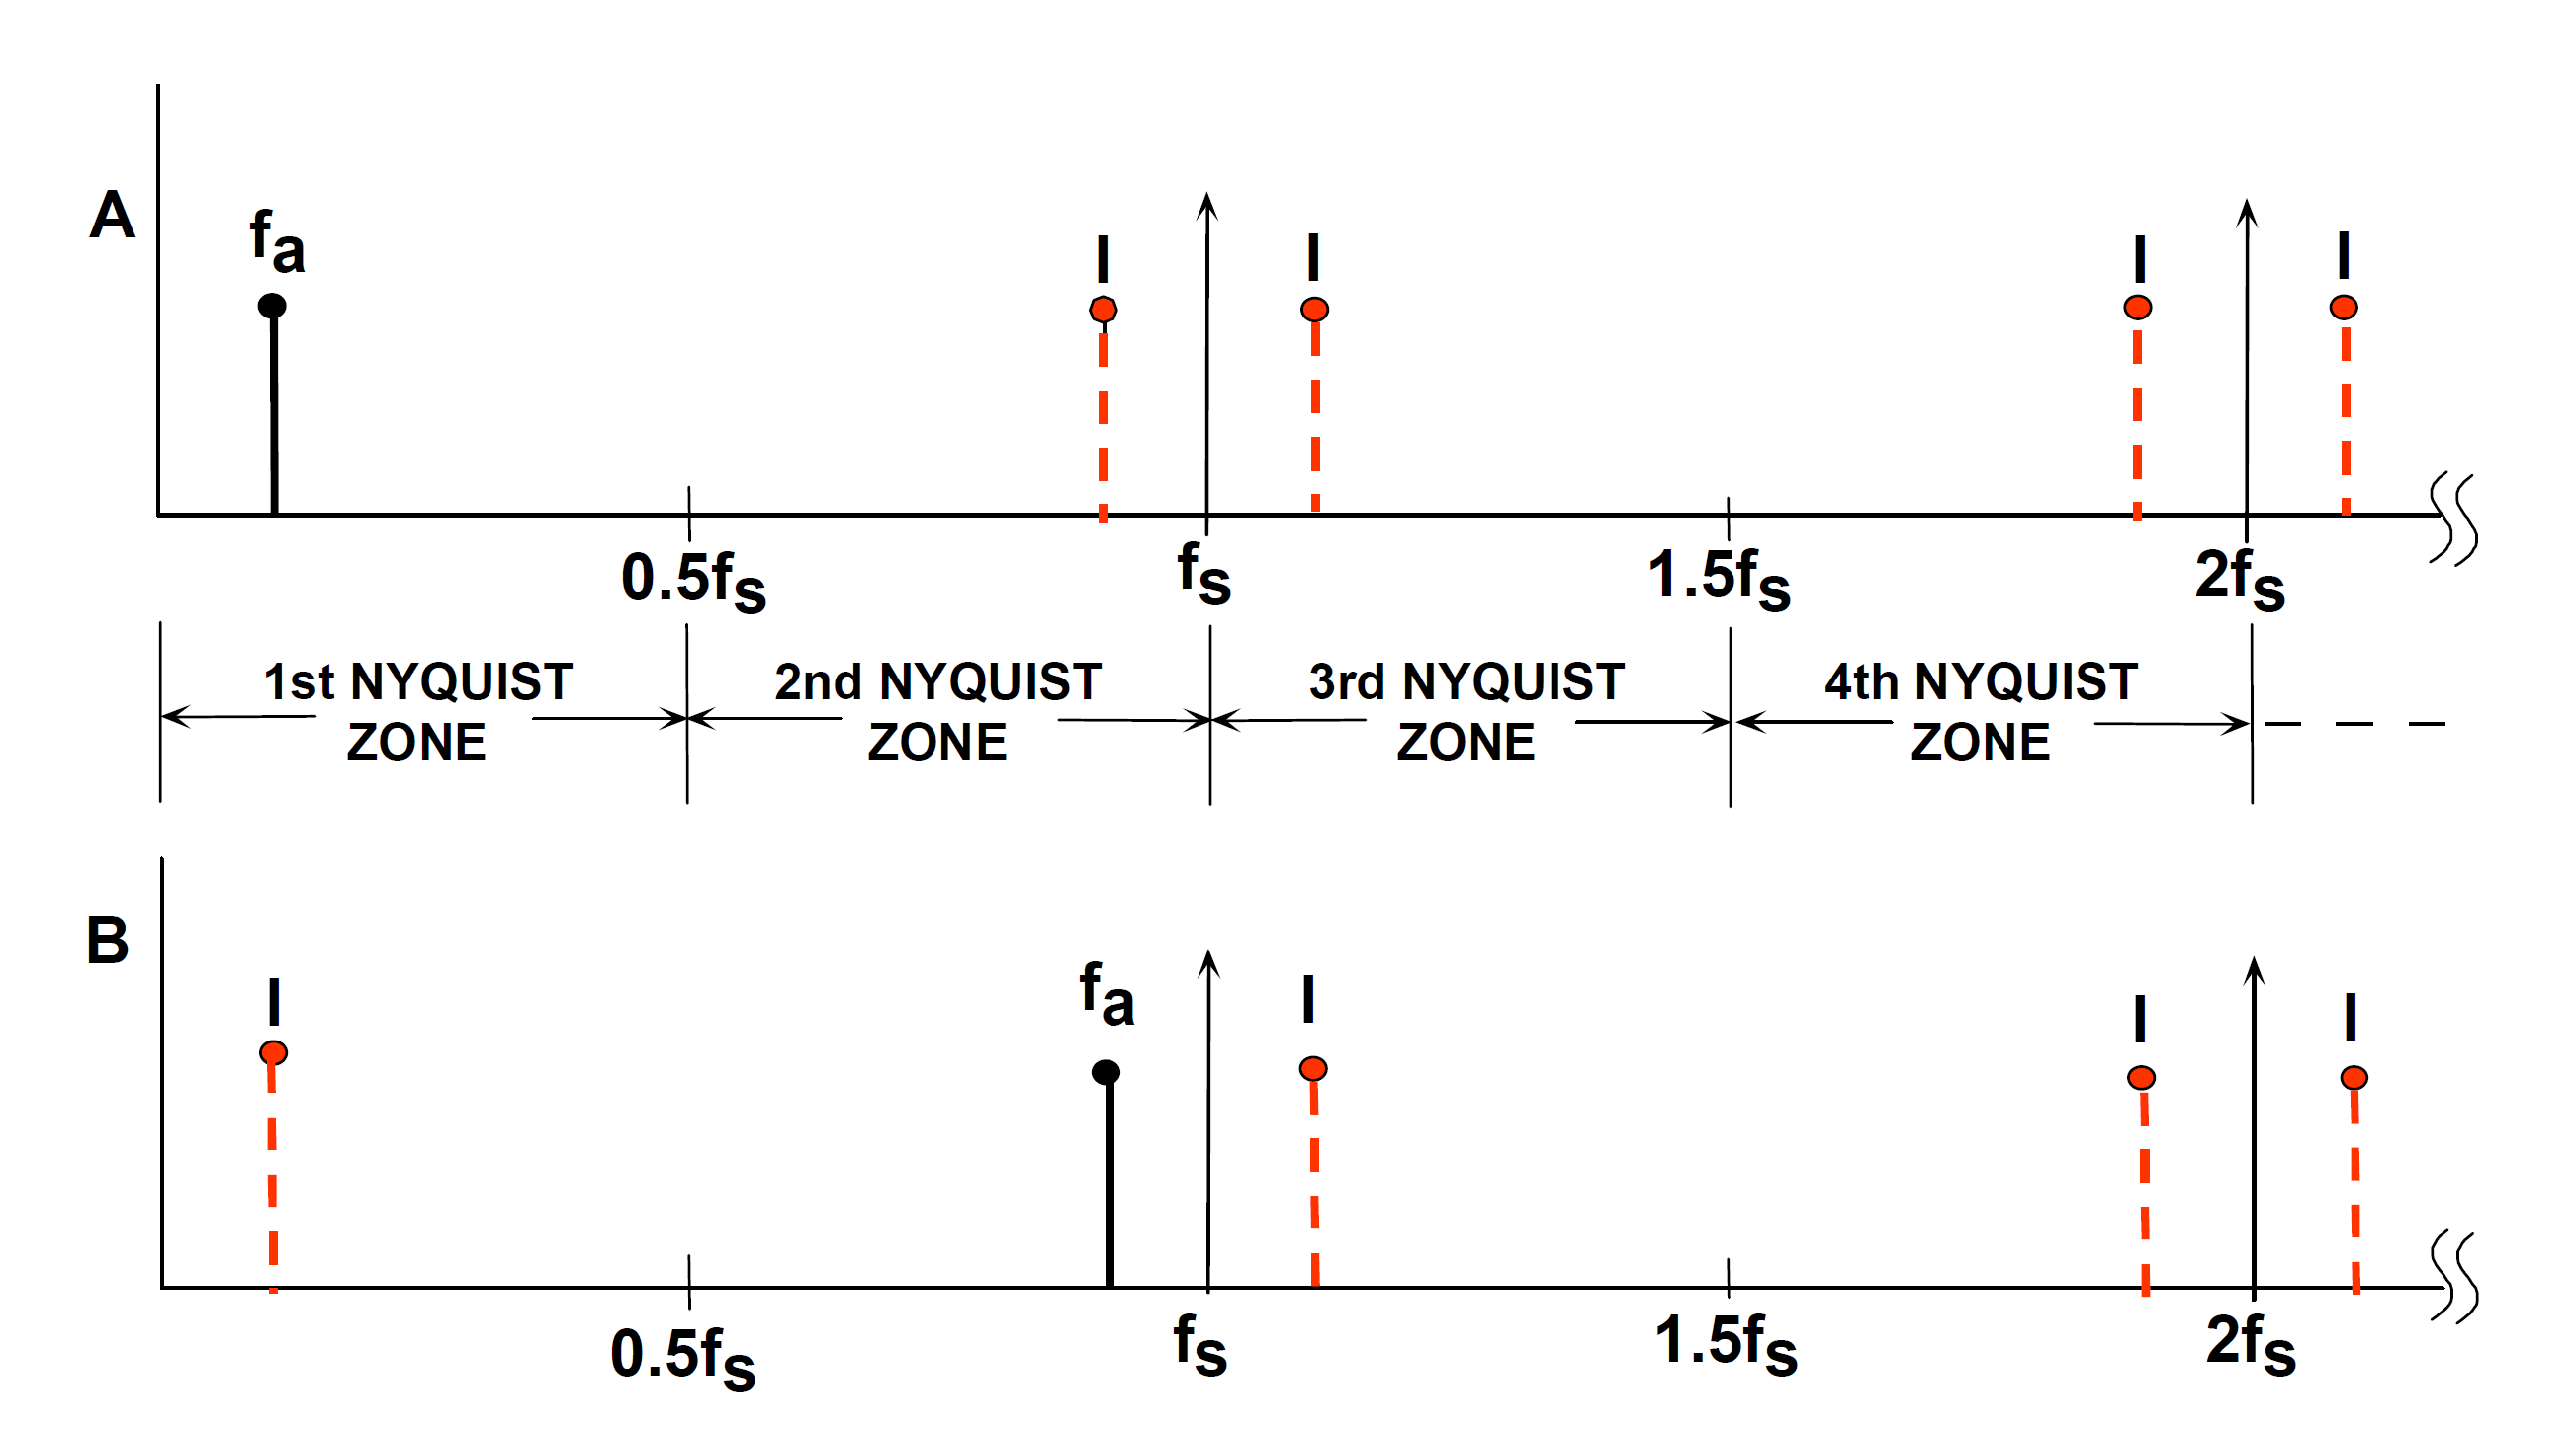
\includegraphics[width=.6\linewidth]{chap/02-theory/img/alias_f}  
		\caption{Sampling in frequency domain}
		\label{fig:alias_f}
	\end{subfigure}
	\begin{subfigure}{\textwidth}
		\centering
		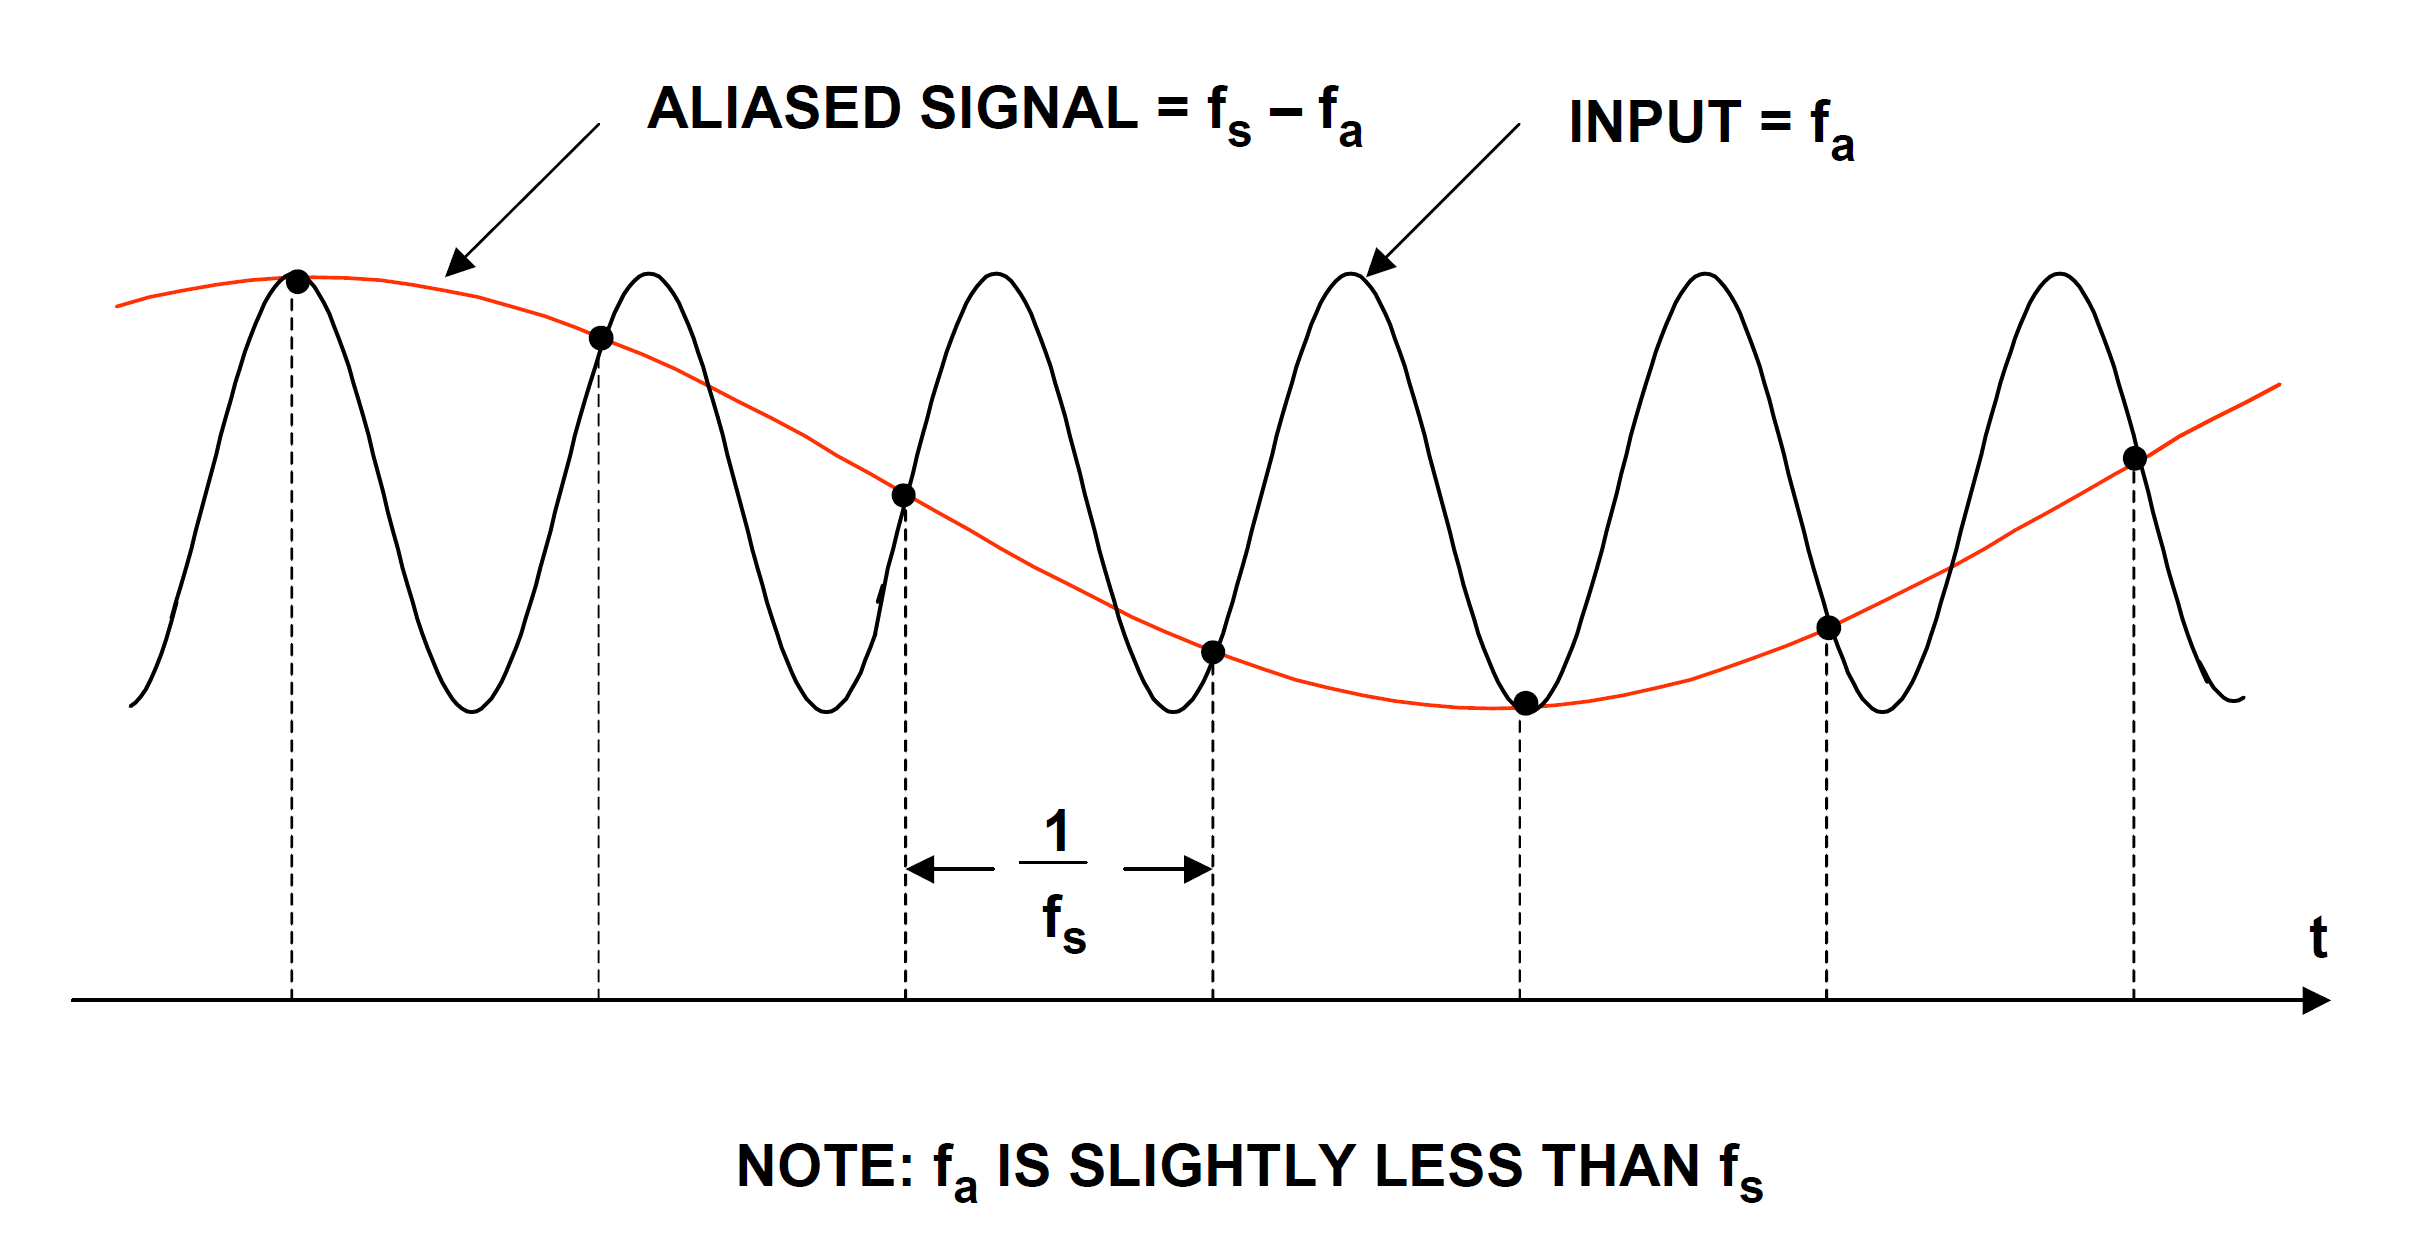
\includegraphics[width=.6\linewidth]{chap/02-theory/img/alias_t}  
		\caption{Aliasing in time domain}
		\label{fig:alias_t}
	\end{subfigure}
	\caption[Aliasing]{Analog signal with frequency $f_a$ sampled at $f_s$ respecting (A) and not respecting (B) the Nyquist criteria. \autoref{fig:alias_t} shows the effect of case B in time domain. \cite{walt}}
\end{figure}

%todo low-pass filter to get B/2<f_s? maybe


\paragraph{Sample-And-Hold-Amplifier}
\Glspl{adc} need a certain amount of time to sample the input signal.
If the level of the analog signal changes by more than one \gls{lsb} during this period, this can result in large errors in the output signal.
Therefore, so called \gls{sha} are used in front of the \gls{adc} to hold the input level constant for the needed amount of time.
The \gls{adc} sampling time needs to be timed in such way, that the analog-to-digital conversion falls into the hold period of the \gls{sha} and does not exceed into the sample period, for example like shown schematically in the diagram below. Thus, the upper frequency limitation is not determined by the \gls{adc} itself, but rather by the aperture jitter, bandwidth, distortion, etc. of the \gls{sha}. \cite{walt}



\begin{figure} [H]
	\centering
	\tikzexternaldisable
	\begin{tikztimingtable}
		[%
		timing/dslope=0.1,
		timing/name/.style={font=\sffamily\normalsize},
		timing/d/text/.style={font=\sffamily\normalsize},
		grayz/.style={timing/z/.append style={gray}},
		timing/n/.style={rectangle},
		timing/metachar={{K}[2]{#1l !{++(0,+.5\yunit)} N[rectangle,scale=.6]{\shortstack{#2}} !{++(0,-.5\yunit)} #1l}},
		timing/metachar={{J}[2]{#1h !{++(0,-.5\yunit)} N[rectangle,scale=.6]{\shortstack{#2}} !{++(0,+.5\yunit)} #1h}},
		]
		SHA & 1H 8K{HOLD} 8J{SAMPLE} 8K{HOLD} 3H\\
		Sampling & 5S A 15S A                    \\
	\end{tikztimingtable}
	\tikzexternalenable
\end{figure}
%todo why not save this as .tikz file and include it as a normal figure with caption?

In addition to the \gls{sha}, there is also the \gls{tha}.
Instead of a sample period, the \gls{tha} has a track period, where the output of the amplifier tracks the input signal (see also \autoref{fig:tha}).
When switching to hold mode, the signal at this instant is held. This is opposed to the \gls{sha}, where the output during sample mode is actually not defined and is set to the value of the input signal, only when switching into hold mode.
%todo explanation a bit confusing. use another timing diagram?

\begin{figure}[tbh]
	\centering
	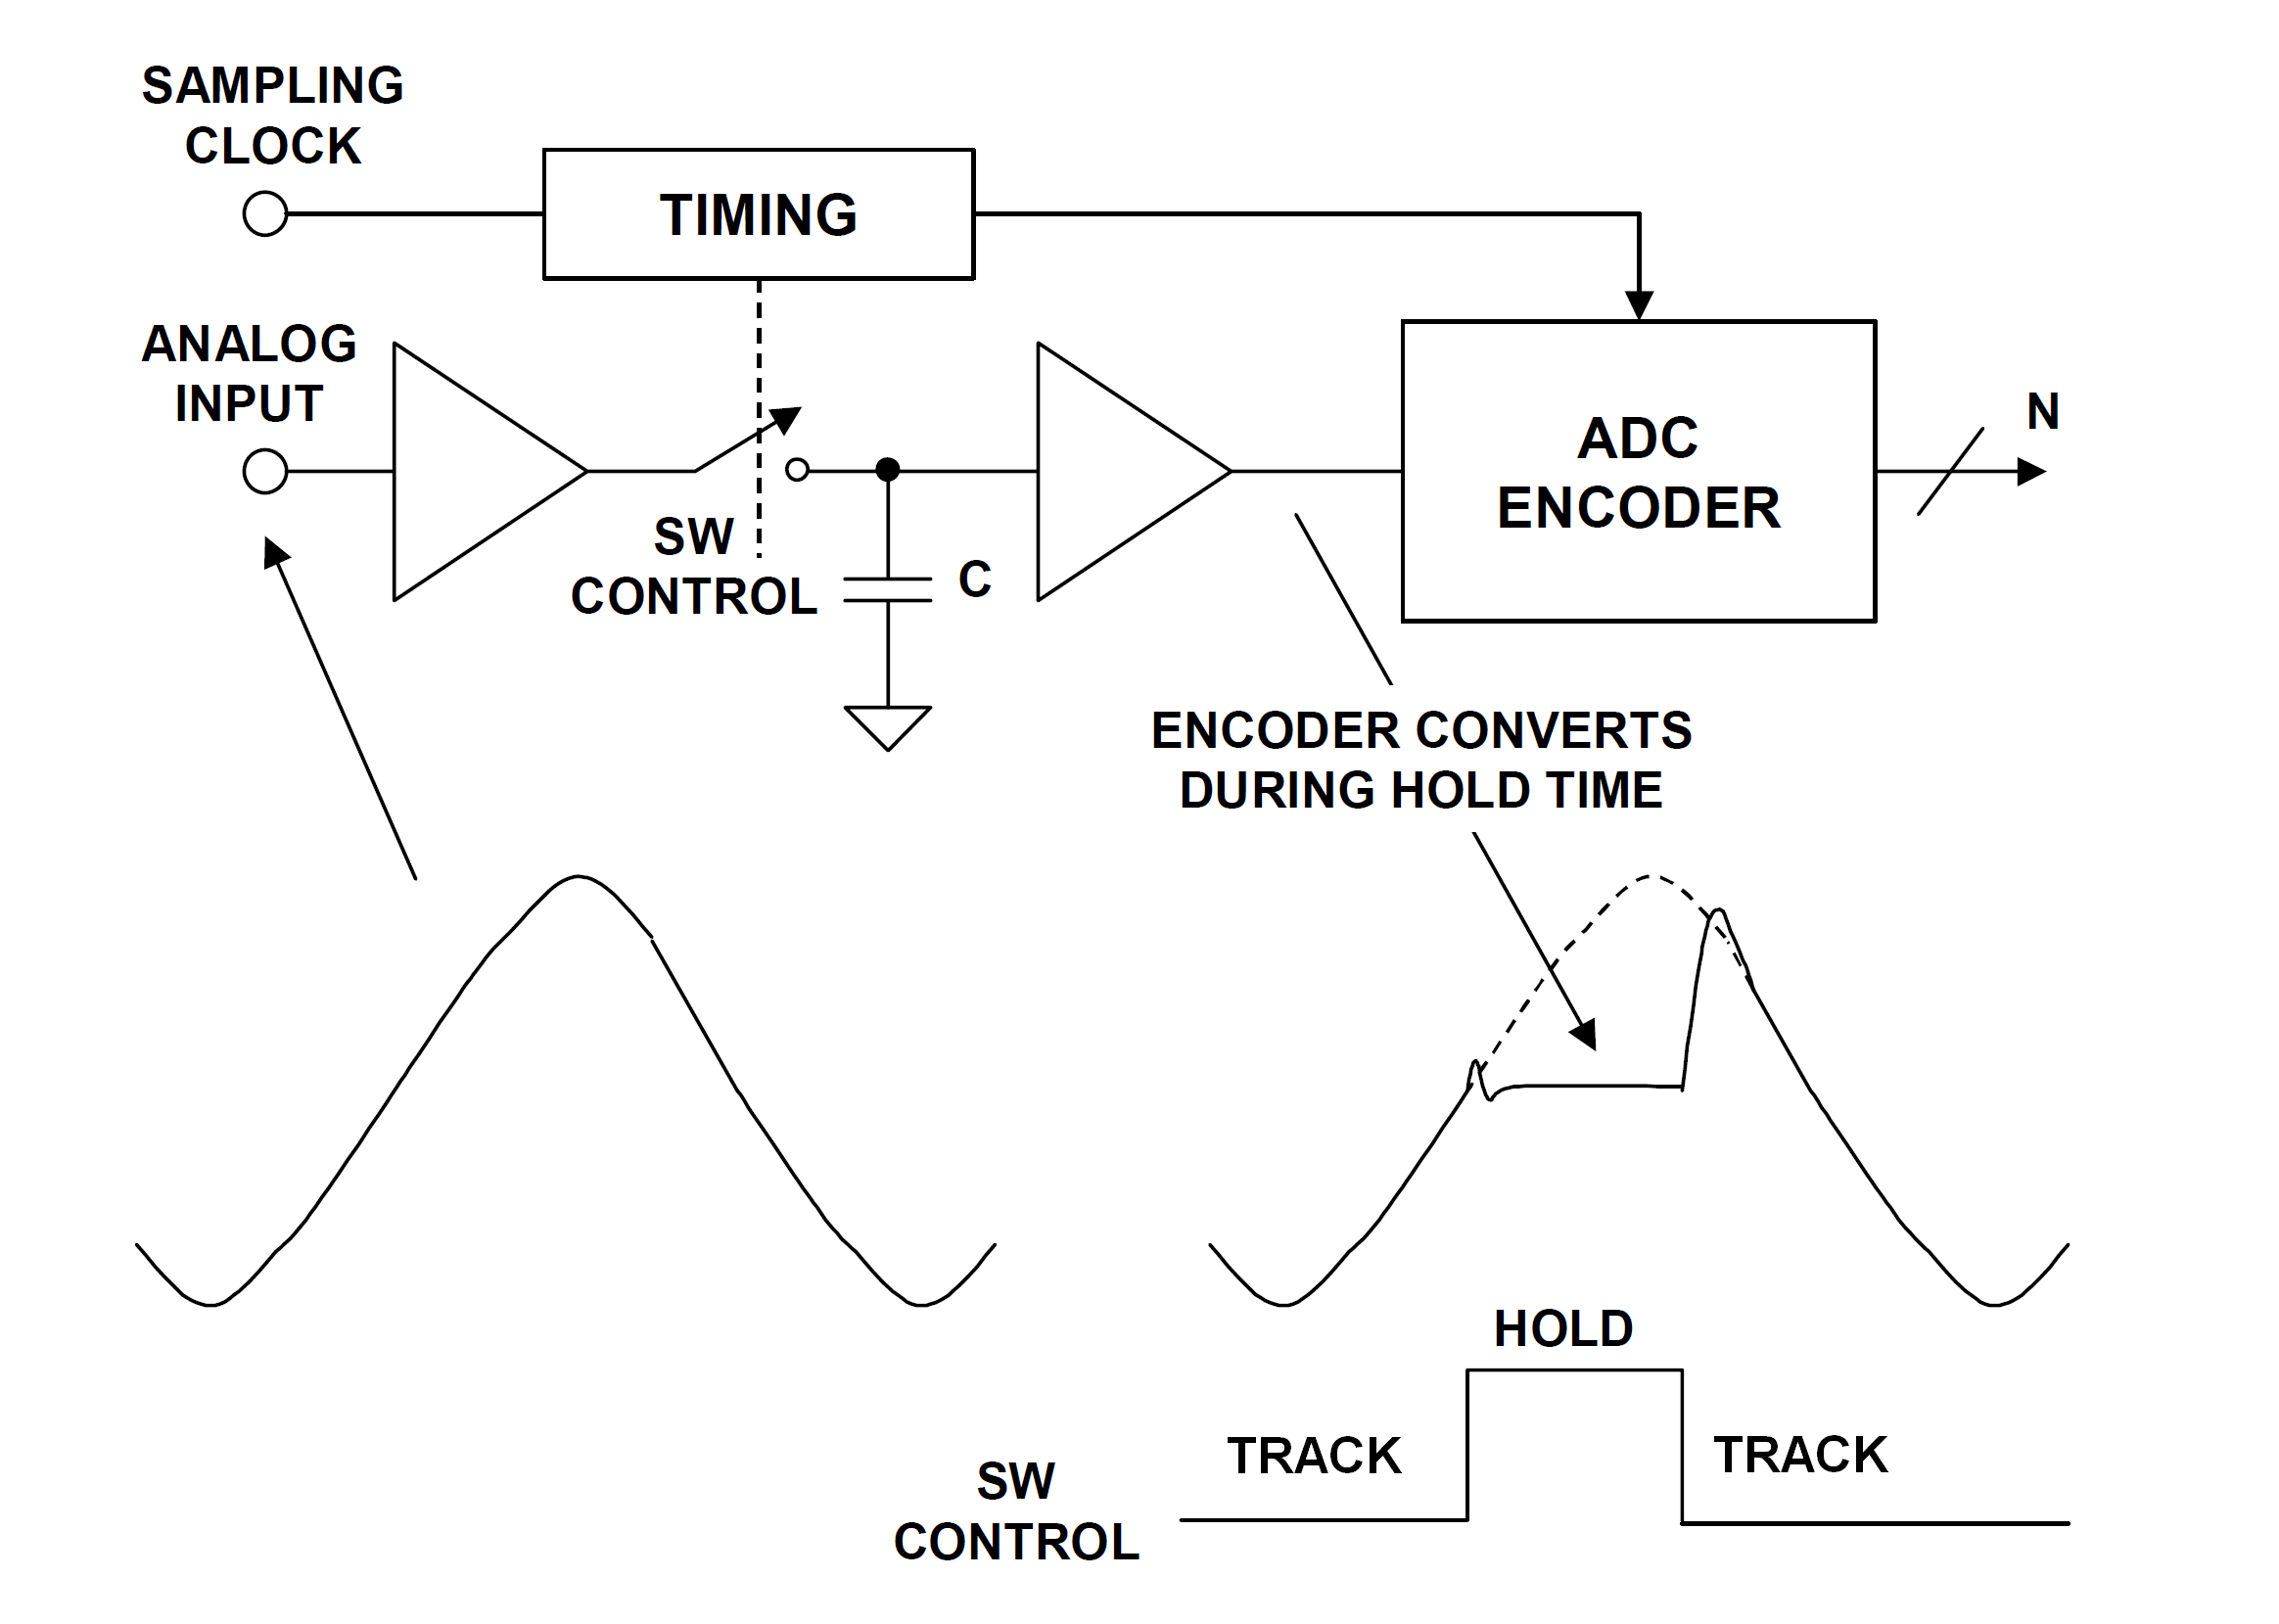
\includegraphics[width = 0.5\textwidth]{chap/02-theory/img/tha}
	\caption{Track-And-Hold-Amplifier schematic and principle \cite{walt}}
	\label{fig:tha}
\end{figure}

\subsection{Characteristics of Analog-To-Digital-Converters}



For an ideal converter, the number of bits would be sufficient to fully characterize it.
Real \glspl{adc} however differ from the ideal behavior by introducing static and dynamic imperfections.
Different applications have different requirements, which leads to a number of specifications. These can be divided into three categories \cite{Lundberg}:
\begin{itemize}[noitemsep]
	\item Static parameters
	\item Frequency-domain dynamic parameters
	\item Time-domain dynamic parameters
\end{itemize}
This section provides an overview of these figures of merit. Which of these are needed to specify the necessary performance of the \gls{adc} has to be chosen for each application accordingly.


\subsubsection{Static parameters}
\textit{Static parameters} are specifications, which can be measured at low speed/DC. 
\paragraph{Accuracy}
\textit{Accuracy} is the total error at a known voltage, which includes:
\begin{itemize}[noitemsep]
	\item Quantization error
	\item Gain error
	\item Offset error
	\item Non-linearities
\end{itemize}

\paragraph{Resolution}
\textit{Resolution} is the number of bits $N$ of the \gls{adc}. Depending from the resolution are the size of the \gls{lsb}, which in its turn determines the dynamic range, code widths and quantization error.

\paragraph{Dynamic Range}
Ratio between smallest possible output (\gls{lsb} voltage) and the largest possible output (full-scale voltage). It can be calculated as
\begin{equation}
	20 \log 2^{N} \approx 6N.
\end{equation}


\paragraph{Offset and Gain Error}
The \textit{offset error} is the deviation of the first transition voltage from the ideal $1/2$ \gls{lsb}. \textit{Gain Error} defines the deviation of the slope of the line going through the zero and full-scale point of the transfer function. These errors can easily be corrected by calibration. Refer to \autoref{fig:offsetErr}

\begin{figure}[H]
	\centering
	\includegraphics[width = 0.55\textwidth]{chap/02-theory/img/offset_err.tikz}
	\caption{Offset and Gain Error in the \gls{adc} characteristic. Notice the difference between the ideal, dotted line}
	\label{fig:offsetErr}
\end{figure}


\paragraph{Integral and Differential Non-linearity Distortion} 
\textit{Integral non-linearity} in the transfer function is the distance of the code centers from the ideal line. It results from the integral non-linearities of the front-end, \gls{sha} and also the \gls{adc} itself. sThese non-linearities depend on the input signal amplitude.

\textit{Differential non-linearitiy} is the deviation in code transition width from the ideal 1 LSB width. This nonlinearity stems exclusively from the encoding process in the \gls{adc}. It not only depends on the input signal amplitude, but also on the positioning along the transfer function.


\subsubsection{Frequency-Domain Dynamic Parameters}

\paragraph{\gls{sinad}}

\begin{itemize}
	\item SINAD
	\item ENOB
	\item SFDR
	\item Total Harmonic Distortion
	\item Intermodulation Distortion
	\item Effective Resolution Bandwidth
	\item Full-Power Bandwidth
	\item Full-Linear Bandwidth
\end{itemize}
\paragraph{Time-Domain}
\begin{itemize}
	\item Aperture Delay
	\item Aperture Jitter
	\item Transient Response
	\item Overvoltage Recovery
\end{itemize}

\subsubsection{Quantization Noise}
Even in an ideal $N$-bit converter there will be errors during the quantization, which behave like noise.
The reason is that each $N$-bit word represents a certain range of analog input values, which is 1 \gls{lsb} wide (\textit{code width}) and centered around a \textit{code center} (see \autoref{fig:idealADC}) \cite{Lundberg}.
The input voltage is always assigned to the code of the nearest code center. 
This means that there will always be a difference between the code center and the actual input.
The difference betweenand the analog input $x(t)$ and its quantized signal $x_q(t)$ is called the \textit{quantization error}.
For an equidistant quantization it is
\begin{equation}
	\left| e_q(t) \right| = \left| x(t) - x_q(t) \right| \leq \frac{q}{2}
\end{equation} 
\cite{puente2015}

Assuming the error voltage uncorrelated and uniformly distributed, the theoretical (maximum) Signal-To-Noise-Ratio (SNR) of this \textit{quantization noise} can be calculated. In the time domain, the quantization error can be approximated with a sawtooth signal \cite{walt}:
\begin{equation}
	e_q(t) = st, \quad -\frac{q}{2s} < t < \frac{q}{2s} 
\end{equation}
%todo why sawtooth? what is 's'? cite?

\begin{figure}[tbh]
	\centering
	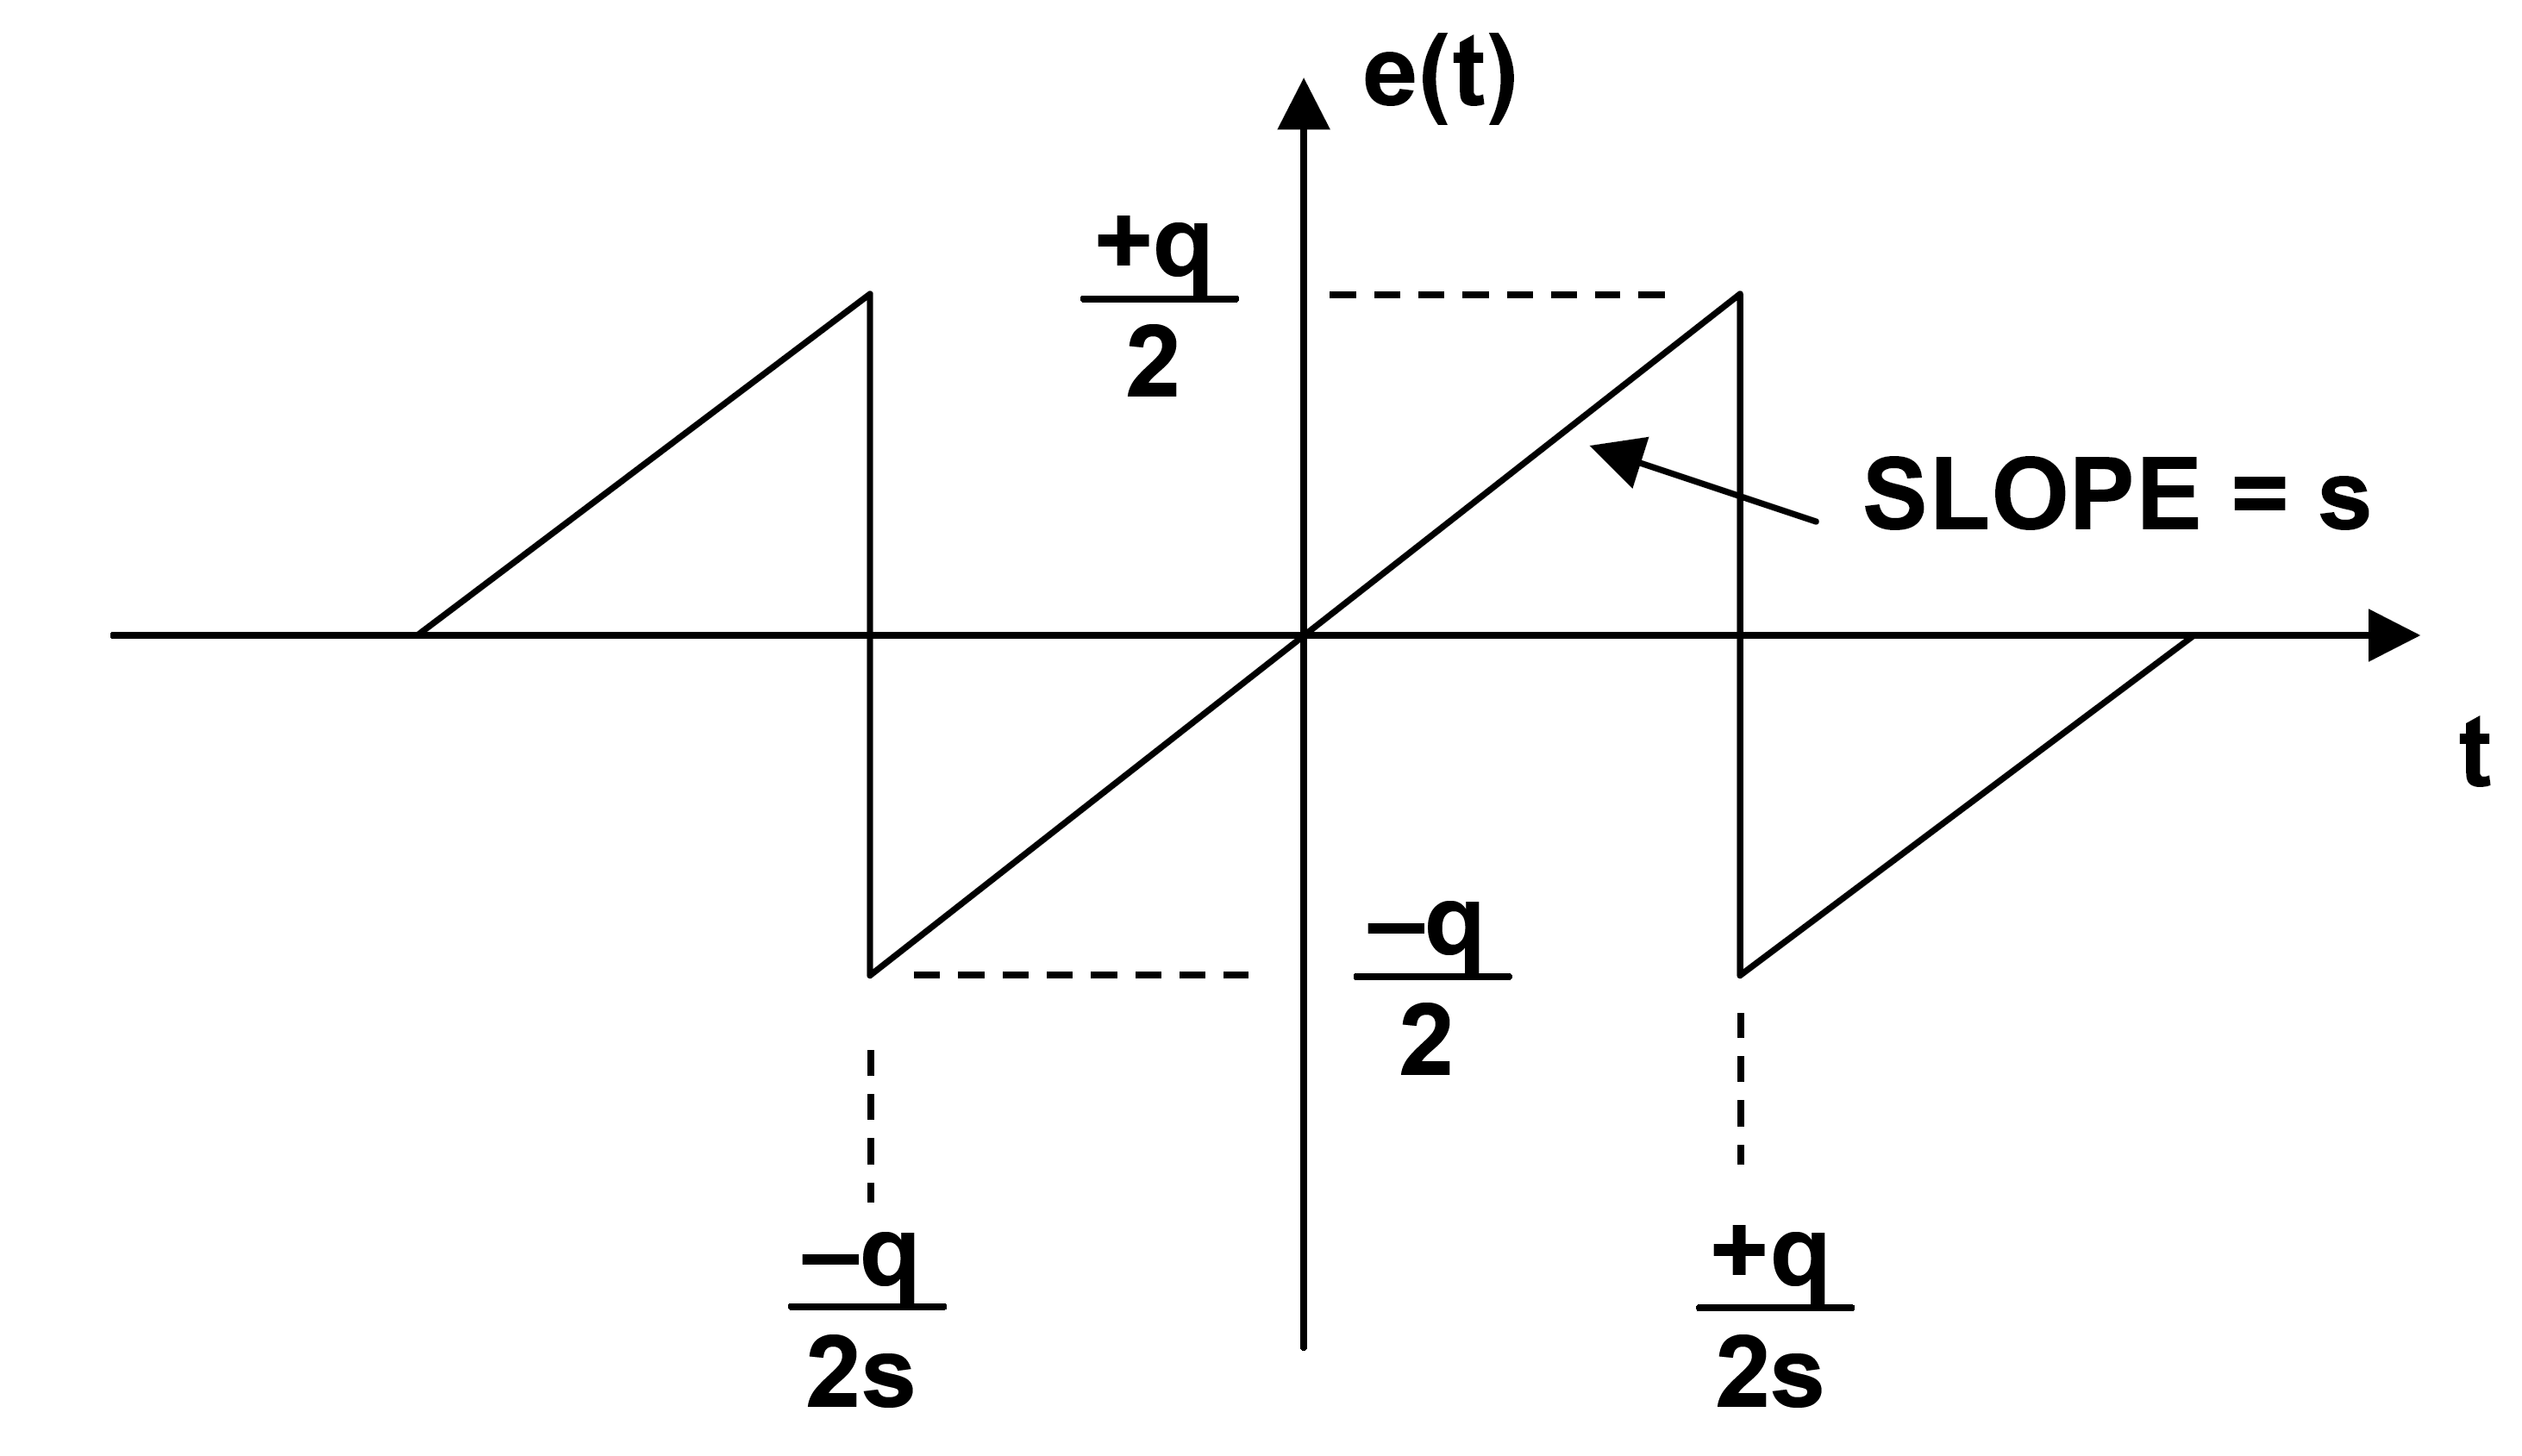
\includegraphics[width = 0.5\textwidth]{chap/02-theory/img/quantization_error.tikz}
	\caption{Quantization noise as function of time (redrawn from \cite{walt})}
	\label{fig:eq}
\end{figure}

%todo how does e relate to e_q?

The power of the quantization noise, which is assumed to be uncorrelated and broadband, can be calculated as the mean-square of $e_q(t)$:
\begin{equation}
	P_\text{QN} = e_{\text{rms}}^{2} = \overline{e^{2}(t)} = \frac{s}{q}\int_{-q/2s}^{+q/2s} (st)^{2} dt = \frac{s^3}{q} \left[ \frac{t^3}{3}\right]_{-\frac{q}{2s}}^{+\frac{q}{2s}} = \frac{q^2}{12}
\end{equation}

To calculate the maximal SNR of an ideal converter, a full-scale input sine wave is assumed:
\begin{equation}
	u(t) = u_s \sin(2\pi f t) = \frac{2^{N}q}{2}\sin(2\pi f t)  = 2^{N-1}q \sin(2\pi f t)
\end{equation}
With the effective value of the signal amplitude
\begin{equation}
	u_{\text{eff}} = \frac{u_s}{\sqrt{2}} = \frac{2^{N-1}q}{\sqrt{2}}
\end{equation}
and the quantization noise power, the SNR can be calculated as
\begin{equation}
	\text{SNR} = \frac{P_{\text{signal}}}{P_{\text{noise}}} = \frac{u_{\text{eff}}^{2}}{e_{\text{rms}}^{2}} = \frac{2^{2N-2}q^2/2}{q^2/12} = 2^{2N} \cdot 1.5.
\end{equation}

Using the unit Decibel, this can be expressed as (see \cite{puente2015,walt})
\begin{equation}
	\text{SNR}|_{\text{dB}} = 10\log\left(2^{2N}\cdot 1.5\right) = 6.02 N + 1.76.
\end{equation}









In an \glspl{adc} (with built-in \gls{sha}) there are a couple of sources, which introduce noise and distortion:
\begin{itemize}
	\item \textbf{Input Stage:} Wideband noise, nonlinearity and bandwidth limitation
	\item \textbf{\gls{sha}:} Nonlinearity, aperture jitter\footnote{\textit{Aperture jitter} is the sample-to-sample variation in aperture delay, with \textit{aperture delay} meaning the time, which is needed by the \gls{sha} to disconnect the holding capacitor from the input buffer.} and bandwidth limitation
	\item \textbf{\gls{adc}:} Quantization noise, integral and differential nonlinearity
\end{itemize}
In the following the most important specifications are described, which are used to characterize the performance of \glspl{adc}.



\paragraph{Equivalent Input Referred Noise}
Internal circuits of wideband \glspl{adc} produce rms noise due to resistor and thermal ("$kT/C$") noise, which is also present for DC signals. Therefore, the output of the \gls{adc} is a distribution of codes which is centered around the value of a DC input. For measuring the value of the noise, the \gls{adc} input is grounded, or held at a specific DC value, and a large amount of samples is collected and plotted as a histrogram. The noise is approximately Gaussian, thus the stndard deviation can easily be calculated.

\paragraph{Noise-Free Code Resolution}
The input referred noise described above determines the \textit{noise-free code resolution}, which is the number of bits, beyodn which it is not possible to resolve individual codes.
\cite{walt}


\subsection{Interleaving}

\begin{itemize}
	\item Net sample rate
	\item Interleaving Spurs
\end{itemize}
